%\documentclass[a4paper,10pt]{paper}
\documentclass{llncs}
\usepackage[utf8]{inputenc}
\usepackage{hyperref}
\usepackage{graphicx}
\usepackage{wrapfig}
\usepackage{listings}
\usepackage{float}
\usepackage{bytefield}
%\usepackage{fullpage}
\usepackage{algorithm}
\usepackage{algpseudocode}
\usepackage{amsmath}
%\usepackage{todonotes}

%opening
\title{LickNet: Software Tools Collection for Guitar Licks Networks}
\author{Matteo Martelli}
\institute{
	University of Bologna\\ 
	\email{matteo.martelli9@studio.unibo.it}
}
\begin{document}

\maketitle

\begin{abstract}
The purpose of the project described in this document is to provide a
method to analyse the relations between musical notes patterns 
in guitar solos.
Given the large amount of guitar solos data available in the Web, it has been possible to
 develop a procedure able to generate a network of guitar solos.
An empirical study has been then conduced in
order to identify some well known characteristic of the generated
networks, turning out that the latter seem to satisfy the small world
property\cite{sw-watts}. Moreover, with the intent to provide an application
for the generated networks, two interesting tools have been developed:
a Licks Classifier, useful to identify at which artist a set of
guitar licks belongs to, and a Licks Generator, useful to create new
licks of a particular guitarist. Despite their ease, these two feature
seem to result very effective.
\end{abstract}
\section{Introduction}
Musicians are often intrigued on how other musicians compose or
improvise their music. A musician also, may often guess if there are some 
relations between its
music and the compositions of other musicians.
Even non expert music enthusiasts often wonder what makes a 
musician unique, well recognisable between the others, or what makes a
musician so similar to another. For example
this frequently happens with guitarists, when people recognize 
a \emph{Santana} guitar solo or a \emph{Hendrix} guitar solo just listening 
 to a few notes of it, or when people
say that \emph{Steve Vai} sounds similar to \emph{Joe
Satriani}.\footnote{\emph{Last.fm}, a
collaborative website, assigns a "super" level of similarity between Steve Vai
and Joe Satriani. This may be related to the fact that Steve Vai was a
his student.}.
One may think that this behaviour is caused by the fact that there are
some notes patterns
repetition in one musician compositions history or that there are some
similar notes patterns between different musicians compositions caused
by their similar musical influence or musical tastes.\\
Thus with the aim to analyse
the relations between notes patterns in guitar
solos, often called guitar licks, the developing process of the software 
described in this
document, \emph{LickNet}, has been started. The choose of guitar solos has been taken 
because of the large amount of data available online but the subject may 
be extended to
different, but similar, kind of data. For example drum patterns
relations in jam sessions or other instruments executions, compositions
and improvisations may be considered. It has been chosen to represent
the data elements and their relations within a network, as to the
means offered by the graph theory useful for a mathematical analysis.\\
The area of scientific research
that usually is interested in the empirical examination of real-world network
 is the study of \emph{Complex Networks}. Some of the study approaches
and mathematical methods that usually interests the Complex Networks
area, such as graph theory or small-world network
comparison\cite{complex-networks}, 
have been considered and will be discussed in the next sections.\\
In addition to the network analysis tools, LickNet provides some other
features like
the \emph{Lick Classifier} and the \emph{Lick Generator}. These
functionalities are still in an early stage but can be a starting point
to realize some practical application focused to end users who may want to
understand and replicate some other guitarist playing style, or to
realize some artificial agents that may ``play'' some music while interacting
with human players.

\section{Related Works}
Several empirical studies about music have been already treated with a
network analysis approach. In \cite{music-genres} networks have been
used to represent the correlations between the musical tastes of
different listener. In addition, the same paper shows a technique to
create a network of musical groups and artists which are connected by
the similarity of their audience; a similar approach has been used in
other remarkable works \cite{artists-network}\cite{metal-network}.\\ 
The authors of \cite{sw-words} introduced a method to create a network of human language words linking
them through a correlation parameter such as their relative distance in
a sentence, assigning the maximum distance for forming link to 2. This
means that two words can be linked together if in a sentence one word is the
successor or the successor of the successor of the other word. They
stated that their choice has two reason:
\begin{enumerate}
\item Many co-occurrences of
words take place at distance of one, e.g. `red flowers' (adjective-noun), 
`stay here' (verb-adverb), `getting dark' (verb-adjective), etc. 
\item Many co-occurrences of words take place at distance of two, e.g.
`hit the ball' (verb-object),
`Mary usually cries' (subject-verb), `Live in Boston' (verb-noun), etc..
\end{enumerate}
In the section \ref{sec:networks} it will be pointed out  
that a similar graph creation procedure as been used in this work, but
with the maximum distance for forming link of 1. This because it is not
trivial
to determine a multi-step correlation value between musical notes in a
notes lick.
Anyway a use of the maximum distance greater than 1 may be tested in future works.

\section{LickNet}
As introduced before, LickNet offers the possibility to study the
relations between notes patterns in guitar solos through the creation
and analysis of guitar licks networks. Moreover it collects
some software tools with which is possible to do some particular
operations with guitar licks through the use of the created networks.
These operations are currently two, a classifier and a generator of
guitar licks.\\
Before getting into the software components, the next section is going
to focus on how the interested data are collected, structured and processed. 

\section{Data Representation}
As many guitarists may already know, there are plenty of websites that
store guitar sheet music files. One of them is \url{www.ultimate-guitar.com}
that counts more than 800000 sheet music files, which are mostly written
with the guitar tablature notation. Guitar players usually choose this
notation for its ease of use \footnote{Guitar tablature removes the
requirement for the player to remember the associations between the
notes and the corresponding fretboard positions, as the latter are directly
represented in the tablature notation.}
but it is instrument-specific. Also, guitar tablature is not standardized and different 
sheet-music publishers adopt different conventions. This means that a
guitar tablature can be understood only by guitar players and its
conversion to the standard notation or formal interpretation may result
wearing. For example the semantic of a guitar tablature changes even if
a guitar it is not standard tuned.\\
Fortunately there are various computer programs available for writing
tablature. One of most frequently used is \emph{Guitar Pro} and the
\emph{Ultimate
Guitar} servers store a large amount of tablature files encoded with its format.
Another interesting software is \emph{TuxGuitar}, a free and open source
tablature editor that also supports the ability to import and export
Guitar Pro files\cite{tuxguitar}. Moreover its source code can be freely
re-used and adapted to any other application. LickNet, in fact, includes
the TuxGuitar library with the purpose of importing the tablature files retrieved
online.\\
After that the tablature can be interpreted by software, a guitar solo
is represented as a sequence of notes, where each of them is composed
 of the following fields:
\begin{itemize}
	\item \textbf{String}: at which string of the guitar the note is played
	\item \textbf{Value}: at which fret of the fretboard the note is played
	\item \textbf{Effects}: a collections of effects such as bending, vibrato,
		harmonic, etc.
	\item \textbf{Duration}: the time duration of the note, represented
as a fraction value.
\end{itemize}
This is how the TuxGuitar library represents the notes, but some
adaptations and additional 
informations are needed for the application purpose. It has been decided
to represent a single note in LickNet as the following:
\begin{itemize}
	\item \textbf{Base Note}: the value of the musical note. It is
a value in the range of [0,12] and not dependent by the octave. The 0th
note is assigned to C, the 11th to B, the last one, and the 12th is the
rest note..
	\item \textbf{Octave}: the octave of the note. The note pitch $p$ is given
by the equation $p = o \times 12 + b $, where $o$ is the octave and $b$
is the base note.
	\item \textbf{Time}: it's a floating point value in the range [0,1] indicating the duration of
the note. The dotted and double dotted notes are also considered, as are
the triplets. For example a quaver dotted note would have a
time value of $\frac{1}{8} + \frac{1}{16} = 0.1875$ and a semi-quaver triplet note
would have the time value of $\frac{1}{16} \times \frac{2}{3} \simeq 0.042$.
	\item \textbf{Bend Distance}: if a note has a bending effect, the bending
distance is the offset from the base note to the bended note. For
example if a F note (base note = 5) is bended to G than the distance is
2, but if it is bended to F\# (half step bending) than the distance is 1. It
is possible that the bending effect is defined with more complex
properties: it may be defined with the \emph{bending and release}
property or with the \emph{bending,
release and bending again} property. Thus it has been decided to calculate
the bending distance has the average bending distance.
	\item \textbf{Node Key}: it is an identifier for a note in the graph. It is
essentially a string where the values of the previous fields, except the
octave, are
concatenated. For instance a semi-quaver triplet F note with a bending
to G would have the resulting node key: ``05:0.042:b2''. There may be the
case in which the bending should not be considered, then the bending distance offset 
will be added to the base note. In this case the node key of the note
used in the
previous example would be: ``07:0.042''.
\end{itemize}

In the next section it will be shown how the data model, here introduced, is used in the
network creation.
\section{Networks Generator}
\label{sec:networks}
%TODO add citations
The network is modeled as a directed multigraph and it's created
scanning the input music sheets files. Let $G$ be a directed
multigraph defined as an ordered 4-tuple $(N,E,s,t)$ with
\begin{itemize}
	\item $N$ a set of nodes,
	\item $E$ a set of edges,
	\item $s: E \rightarrow  N$, assigning to each edge its source node,
	\item $t: E \rightarrow N$, assigning to each edge its target node.
\end{itemize}
Moreover a node $n \in N$ contains a musical note identified by its Node Key.
An edge $e \in E$ from a node $s$ to a node $t$ exists if the musical note
contained in the node $t$ was a successor, in the input music sheet, of the musical note 
contained in the node $s$. Also, there may exists more than one edge from a node $s$ and $t$
as a same musical note can be reached by another note many times with
different octaves jumps. Thus an edge from $s$ to $t$ indicates with which
octave jump the note contained in $s$ can reach $t$ in a graph walk step.
An example of a multigraph with its corresponding sheet music is shown
in figure \ref{fig:multigraph}.
\begin{figure}
\centering
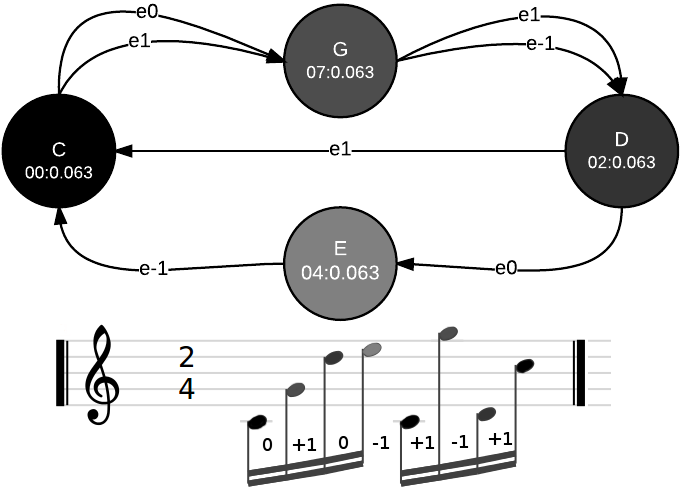
\includegraphics[scale=0.4]{multigraph.png}
\caption{A multigraph example. The corresponding input data used for the multigraph
creation is represented with its sheet music. The id of each edge
indicates with with octave jump its source node can reach the target
node.}
\label{fig:multigraph}
\end{figure}
The octave informations are not included in the graph nodes because 
similar licks can be played at different octaves and otherwise it would be
harder to underline the relations between them.\\
It has been decided to add a weight to each edge that corresponds on the
times that an edge is passed through. This means that many walks
from a node $a$ to a node $b$ with the same distance $d$ but different
total weight exist in the graph, and the walk that more likelihood
correspond to a significant lick for the graph is the one with the
highest total weight. A lick is intended to be significant if it is
similar to the licks that are already used in the graph creation. The
process that determines if a lick is significant for a certain graph will
be covered in the next section.\\
A simplification of the model has been introduced in the development
process: the directed multigraph is represented as a directed graph,
where an edge is an object that contains an array which each element $i$
indicates the pass-through frequency number for the octave corresponding
to $i$. More specifically if $f(j)$ is the frequency number related to the
octave jump $j$, then 
\[ v(i) = f(i + n), \]
where $n$ is the maximum octave increment or decrement possible.
All the octaves on a standard tuned guitar are 5, thus with 6 octaves even
the 7-strings guitars and most of the non-standard tuned guitars can be
covered. Therefore the size of the array is 12 as a node $s$ can reach
in a single step a node $t$ with an increment or decrement of most 6
octaves. To clarify, for example if the node $s$ has reached with a
single step the node
$t$ 5 times without any octave jump, 3 times with an octave jump of +1, 
1 time with an octave jump of +2
and 2 times with an octave jump of -1, the resulting octave jumps array
for the edge $e$ that connects $a$ and be would be:
\[ v = (0,0,0,0,0,2,5,3,1,0,0,0,0) \]
 A directed edge $e$ from $s$ to $t$ exists if at least one
element of the array is non-zero.
The algorithm \ref{algo:gcreation} shows how the graph creation process
works.
\begin{algorithm}
\caption{Graph creation algorithm}
\label{algo:gcreation}
\begin{algorithmic}[1]
\Function{createGraph}{$sheets$}
	\State $G \gets $ emptyGraph()
	\For {$s$ in $sheets$}
		\For {$n$ in $s.notes$}
			\If {$pn$} 
				\State $S_k \gets $ genNodeKey($pn$)
				\State $T_k \gets $ genNodeKey($n$)
				\If {$S_k \notin G$.nodes }
					\State createNode($G$, $S_k$)
				\EndIf
				\If {$T_k \notin G$.nodes }
					\State createNode($G$, $T_k$)
				\EndIf
				\State $E_k\gets A_k + B_k$ 
					\Comment{\scriptsize{Strings concatenation}}
				\small
				\If {$E_k \notin G$.edges }
					\State createEdge($G$, $E_k$)
				\EndIf
				\State $e \gets$ getEdge($G$, $E_k$)
				\State $ojump \gets n$.octave - $pn$.octave 
				\State $id \gets ojump$ + N\_OCTAVES
				\Comment{\scriptsize{N\_OCTAVES is 6 for a guitar}}
				\small
				\State $e$.ojumps[$id$] += 1
			\EndIf
			\State $pn \gets n$
		\EndFor
	\EndFor
\EndFunction
\end{algorithmic}
\end{algorithm}

\subsection{Networks Analysis}
\begin{figure}[H]
\centering
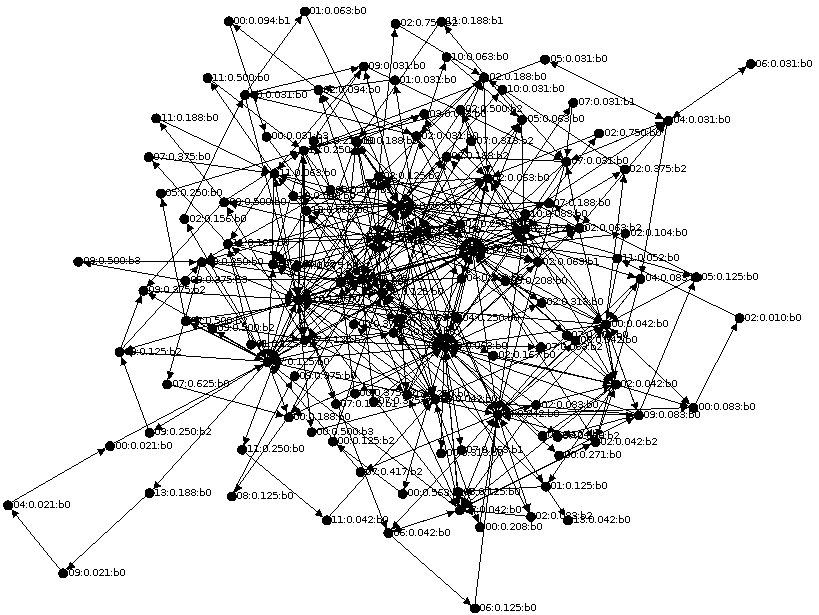
\includegraphics[scale=0.43]{hendrix_graph.png}
\caption{A graph example created with 6 Jimi Hendrix
solos. Edges of self linked nodes are not shown.}
\label{fig:hendrixgraph}
\end{figure}
The figure \ref{fig:hendrixgraph} shows a graph created with the
algorithm \ref{algo:gcreation} using 6 Jimi Hendrix solo files as input.
The resulting graph counts 124 nodes and 484 edges and the bending
effects has been considered. Interestingly, the same graph created
without the bendings consideration counts 101 nodes. This seems to
happen also with other graphs and the difference is higher with those
guitarists that heavily use bendings. This suggests that 
considering more 
guitar effects, such as vibratos or virtual harmonics, 
the vertex cardinality tends to increase. In the next
sections it will be shown that considering more guitar effects may be 
also interesting for the
licks classifier and the licks generator.

Many research articles on real network graphs, like biological, 
social and technological graphs showed that they share a common
feature: the so-called small-world (SW) property \cite{sw-watts}.
In SW networks most nodes can be reached from every other by a small
numbers of steps and furthermore they are characterized by a high
clustering coefficient. In order to verify if the networks of guitar
licks respects the SW properties, the average clustering coefficient $C$ and the
average shortest path length $L$ must be determined\cite{sw-ubiquity}. In this analysis
the network is converted to a non-directed graph as a model
simplification. Let us start defining 
the clustering coefficient: given $e_{ij}$ an edge from the vertex $v_i$
to the vertex $v_j$, the number of cycles of length 3 (closed triplets) from/to a node $i$ is:
\[ p_{ii}^{(3)} = \sum_{jk}[Maw{e_{ij}e_{jk}e_{ki}}\;, \]
thus the local clustering coefficient of a node $i$ is 
\[ C_i = \frac{p_{ii}^{(3)}}{k_i(k_i-1)/2} \; ,\]
and the average clustering coefficient of a graph is
\[ C = \frac{1}{N} \sum_{i}{C_i} \;  \]
where $N$ is the number of nodes in the graph.
Moreover the shortest path length average $L$, is defined as:
\[ L = \frac{1}{N(N - 1)} \sum_{i,j,i \neq j}{d_{ij}} \]
where $d_{ij}$ is the shortest path length from a node $i$ to a node
$j$.
Then the table \ref{tab:sw} shows the $C$ and $L$ values of some graphs created with the algorithm
\ref{algo:gcreation} and converted to non-directed graphs, the $C_{rand}$
and $L_{rand}$ values that indicates $C$ and $L$ of the equivalent
derived random networks and the small-coefficient $\sigma$ defined as:
\[ \sigma = \frac{C / C_{rand}}{L / L_{rand}} \]

What is remarkable is that the $\sigma$ values are $> 1$, also $C \gg
C_{rand}$ and $L \approx L_{rand}$, satisfying the SW property
\cite{sw-ubiquity}.
\setlength{\tabcolsep}{8pt}
\begin{table}
\begin{center}
  \begin{tabular}{ l c c c c c c  }
    \hline
    graph  & $N$ & $C$ & $C_{rand}$ & $L$ & $L_{rand}$ & $\sigma$ \\ \hline
    Dave Murray & 102 & 0.329 & 0.074 & 2.864 & 2.602 & 4.039 \\
	Jimi Hendrix & 124 & 0.429 & 0.064 & 2.675 & 2.649 & 6.63 \\
	Angus Young & 122 & 0.266 & 0.068 & 3.092 & 2.888 & 3.65 \\ 
	Whole Graph & 213 & 0.531 & 0.049 & 2.734 & 2.627 & 10.4 \\
    \hline
  \end{tabular}
\end{center}
  \caption{Small World comparison results. Each graph is created with
the tablature files of a particular guitarist except for the Whole Graph
that is created with all the tablature files used for the other graphs
generation.}
  \label{tab:sw}
\end{table}
 
\section{Licks Classifier and Generator}
As introduced before, a possible application for the graphs created with
the method described in the previous section may be a lick classifier.
Let us introduce the scenario in which a graph is created with the solos
of a particular guitarist only. Then, creating a graph for different
guitarists, it may be tempting to identify to which of them an unknown
guitar lick belongs to. This can be possible because the links in the
graphs are weighted according to the number of times they are walked
through, meaning that if a sequence of musical notes results having
a higher 
total weight in a walk on a graph $a$ than on a graph $b$, the probability that the sequence 
occurs more often on the graph $a$, and in the
corresponding guitarist solos, than on the graph $b$ is also higher.
With this idea the lick classifier works: from a set of graphs and one
lick it simply performs a walk of the lick on every graph collecting the
corresponding total weights. The total weights are then dived by the
number of notes used in the corresponding graphs creation.

Another proposed application is the Licks Generator: through the "LickNet" user
interface, it is possible to select a graph from the graphs list and
generate a set of licks, which is sorted in a descending ordered by
the matching score of the licks. Its algorithm is very simple: first it
performs a very big number of random walks on the selected graph. Each
of the walk has a resulting total weight with which the generator is
able to sort them. Only the first $N$, with $N$ as a small number, 
licks are then considered to be significant for the selected graph.

It will be shown in the next section that even if the two applications
described here are very simple, they can be effective.

\section{Tests and Results}
The table \ref{tab:classifier} shows the results of 4 tests
made with the lick classifier. For convenience let us call
\emph{library} the set of graphs used the experiments. Every graph of
the library has been generated from a set of solos of a particular
guitarist, more precisely Jimi Hendrix, Dave Murray and Angus Young.\\
For each experiment it has been classified a
guitar solo (licks set) of a particular guitarist that was not used in
any of the graph creation (unknown). 
Each row indicates a different
experiment, the first column indicates the guitarists of the unknown
licks set used
for each experiment and the remaining columns indicate the scores gained
for each graph by the corresponding unknown licks set. \setlength{\tabcolsep}{8pt}
\begin{table}
\begin{center}
  \begin{tabular}{ l c c c }
    \hline
    Lick guitarist  & Dave Murray & Jimi Hendrix & Angus Young  \\ \hline
	Jimi Hendrix & 0.285 & \underline{\textbf{0.356}} & 0.196 \\
    Dave Murray & \underline{\textbf{0.268}} & 0.052 & 0.040 \\
	B.B. King & 0.011 & \underline{\textbf{0.057}} & \textbf{0.045} \\
	Kirk Hammett & \textbf{0.724} & \underline{\textbf{0.785}} & 0.403 \\
  \end{tabular}
\end{center}
\caption{Licks classifier test results.}
\label{tab:classifier}
\end{table}

Moreover the scores are relative to each test and should not be
interpreted globally, as they are dependent on the notes sequence
length of the licks.
It is interesting how well the classifier recognizes that an unknown
licks set of a guitarist in the library belongs to its guitarist. What
is also remarkable is that the matching expectation of the experiments are 
satisfied: without any surprise, the licks set of B.B. King 
matches more the graph of Jimi Hendrix than the others. Also it is not
very far the score of Angus Young while it is the score of Dave Murray.
This may be caused by the fact that Jimi Hendrix and Angus Young may be
more influenced by the blues playing style. Furthermore it may result
weird that the licks set of
Kirk Hammett, the lead guitarist of Metallica, matches more the Jimi
Hendrix graph than the others. But the thing to notice is that the score
matching with Dave Murray is also close while the score with Angus Young
is far. This may be caused by the fact that Hammett was influenced by
Jimi Hendrix \cite{hammet-hendrix} in his early years and that the genre played by Metallica
is closer to the genre played by Iron Maiden. Anyway these are all
suppositions, for a better interpretation it can be helpful considering the
graph of Kirk Hammett also, in order to determine the gap between those
scores and the score gained with Kirk Hammett himself. For example by the
first two experiments one may interpret that Jimi Hendrix has a closer
relation with Dave Murray than Angus Young, but with the limited amount
of data this cannot be easy verified. A measurement method for finding the
correlations between the guitarists using the classifier here proposed
may be modeled in future works.


With the same library, the Licks Generator has been tested. For every
guitarist it has been generated a set of licks that it has been tested
again with the lick classifier in order to see if the generated licks
can be significant for the respective guitarists. As expected, each set
of generated licks gains the best score with its corresponding
guitarist.\\
In addition, in the LickNet source code repository\footnote{The
repository is currently located at
\url{https://github.com/matteomartelli/licknet}. Also all the software
parts are free software and the source code is open. The instructions
for contributing are provided in the README file.}
 provided with this document,
there is an example data folder that contains the tablature files used
to generate the library, the tablature files of the licks used in the
classifier tests and the tablature files of the licks created with the
lick generator.
\begin{table}
\begin{center}
  \begin{tabular}{ l c c c }
    \hline
    Lick guitarist  & Dave Murray & Jimi Hendrix & Angus Young  \\ \hline
	Jimi Hendrix & 0.220 & \underline{\textbf{0.323}} & 0.069 \\
    Dave Murray & \underline{\textbf{0.293}} & 0.208 & 0.052 \\
	Angus Young & 0.117 & 0.131 & \underline{\textbf{0.449}} \\
  \end{tabular}
\end{center}
\caption{Results of the generated licks tested on the Licks Classifier.}
\label{tab:classifier}
\end{table}

\section{Future Development}
In this section it will be proposed some enhancement to the software.
The first one is to find a method to automatically retrieve and
reorganise the tablature files. The main problem is that those files are
often badly written and mostly without the key signature indication. As
an automatic method such this one can be hard to develop, another solution
may be to provide a public database of tablature files already
reorganised for LickNet by their users.
As already introduced before, a second enhancement can be a feature for
co-relating the artists within their licks: it may works with the
classifier that from a set of licks of an artist can relate the latter
to the other artists in the library by the score gained for each
corresponding graph.\\
Moreover this software may be attached to other projects: for example it may be used 
in an improvisation software to generate runtime the notes of the
soloist musician, or it may be attached to some tablature editor to easy
generate some licks as start points for user compositions.

\section{Conclusions}
In the interests of the complex network analysis, it has been seen that
the networks of licks seem to be organised with the properties of small
world networks. Furthermore, these networks look like to have a
structure that highly depends from the input data used in their
creation and from their corresponding guitarists. Therefore, functions
that operates on the guitarists signature playing style, such as the
licks classifier and the licks generator, stand to reason.

The initial expectations are well satisfied and LickNet appear to be a
good start point for developing a various amount of software related to
music classification and composition.

\begin{thebibliography}{50}
	\bibitem{complex-networks} 
		Maarteen van Steen, 
		\textsl{Graph Theory and Complex Networks: An Introduction}, 
		2010.
	\bibitem{music-genres}
		R. Lambiotte, M. Ausloos,
		Uncovering collective listening habits and music genres in bipartite networks,
		\textsl{Phys. Rev. E 72, 066107},
		2005
	\bibitem{artists-network}
		Dr Tamás Nepusz,
		Reconstructing the structure of the world-wide music scene with Last.fm,
		http://sixdegrees.hu/last.fm
	\bibitem{metal-network}
		Benjamin Lind,
		Patterns in the Ivy: The Small World of Metal,
		http://badhessian.org/2013/09/patterns-in-the-ivy-the-small-world-of-metal/,
		2013
	\bibitem{sw-words}
		Ramon Ferrer i Cancho, Ricard V. Solè,
		The small world of human language,
		\textsl{Proc. Royal Soc. London B, DOI: 10.1098/rspb.2001.1800}
		2001
	\bibitem{tuxguitar}
		Daniel Mantilla,
		TuxGuitar: Editorial review,
		\textsl{Software Informer},
		2014.
	\bibitem{sw-watts}
		Watts, D. J. and Strogatz, S. H.,
		Collective dynamics of `small-world’ networks,
		\textsl{Nature 393, 440-442},
		1998
	\bibitem{sw-ubiquity}
		Qawi K. Telesford, Karen E. Joyce, Satoru Hayasaka, Jonathan H. Burdette, Paul J. Laurienti
		The Ubiquity of Small-World Networks,
		\textsl{Brain Connect.; 1(5): 367–375},
		2011
	\bibitem{hammet-hendrix}
		Brian Ives,
		Hendrix At 70: “My Favorite Guitar Player Of All Time” – Kirk Hammett Of Metallica,
		\textsl{CBS Local},
		http://wcbsfm.cbslocal.com/2012/11/25/hendrix-at-70-my-favorite-guitar-player-of-all-time-kirk-hammett-of-metallica/,
		2012
	\end{thebibliography}
\end{document}
